\chapter{Analyse et spécification des besoins}

\section{Introduction} 
Dans ce deuxième chapitre, nous allons approfondir l’étude de notre projet en analysant ses éléments clés. Nous débuterons par une identification des différents acteurs impliqués ainsi que des fonctionnalités qui leur sont attribuées. Par la suite, nous préciserons les besoins fonctionnels et non fonctionnels de l’application. Nous illustrerons ensuite l’ensemble des interactions à travers un diagramme de cas d’utilisation et établirons le backlog produit. Enfin, nous détaillerons l’architecture globale du système ainsi que l’environnement technique dans lequel il sera développé.

\section{Analyse des besoins}

\subsection{Identification des acteurs}
On définit un acteur comme toute entité qui joue un rôle actif et interagit avec l’application. Dans cette partie, nous soulignons les acteurs majeurs qui participent au fonctionnement de notre système :

\begin{table}[H]
    \centering
    \renewcommand{\arraystretch}{1.3}
    \begin{tabular}{|p{3cm}|p{10cm}|}
        \hline
        \textbf{Acteur} & \textbf{Description} \\
        \hline
        Admin & Il supervise la gestion des utilisateurs et des organisations pour assurer un accès sécurisé et un fonctionnement optimal de l'application. Il veille à la stabilité du système et à l'amélioration continue de la plateforme. \\
        \hline
        Utilisateur & Il représente un utilisateur qui peut s'inscrire, se connecter, gérer son profil, consulter les alertes, examiner les suggestions de l'IA, et consulter les erreurs et journaux générés pour surveiller les anomalies. \\
        \hline
    \end{tabular}
    \captionsetup{justification=centering}
    \caption{Identification des acteurs}
    \label{tab:actors}
\end{table}

\subsection{Besoins fonctionnels}
Les besoins fonctionnels décrivent les fonctionnalités spécifiques que l'application doit fournir. Ils sont directement liés aux actions que l'utilisateur peut effectuer. Voici les besoins fonctionnels identifiés :

\begin{itemize}[label=\textbullet]
    \item \textbf{Authentification :} Inscription, connexion, vérification et réinitialisation du mot de passe.
    \item \textbf{Gestion des utilisateurs :} Permet aux super administrateurs de gérer les utilisateurs.
    \item \textbf{Gestion des organisations :} Ajout, suppression et modification des organisations par les administrateurs.
    \item \textbf{Gestion des pipelines :} Création, modification et suppression des pipelines.
    \item \textbf{Gestion du profil :} Modification des informations personnelles par les utilisateurs.
    \item \textbf{Tableau de bord :} Affichage des données personnalisées pour les utilisateurs.
    \item \textbf{Consultation des logs et metrics :} Analyse des données de logs et métriques.
    \item \textbf{Erreurs détectées :} Suivi des anomalies identifiées par le système.
    \item \textbf{Suggestions IA :} Recommandations fournies par l’IA.
    \item \textbf{Discussion IA :} Interaction avec ChatGPT, Gemini, Llama 3.
\end{itemize}

\subsection{Besoins non fonctionnels}
Les besoins non fonctionnels définissent les contraintes et critères de qualité que le système doit respecter, indépendamment de ses fonctionnalités principales. Ils assurent la robustesse, la sécurité, et la performance globale de l’application.

\begin{itemize}[label=\textbullet]
    \item \textbf{Simplicité :} 
    L'interface utilisateur doit être claire, intuitive et ergonomique, permettant à tout utilisateur, même non technique, de naviguer facilement et d’accéder rapidement aux fonctionnalités principales sans nécessiter de formation particulière.
    
    \item \textbf{Performance :} 
    Le système doit être capable de traiter les demandes des utilisateurs en temps réel ou quasi temps réel. Les opérations critiques, telles que l’analyse des logs ou la récupération des données depuis la base ElasticSearch, doivent être optimisées pour réduire au maximum le temps de latence.
    
    \item \textbf{Évolutivité :} 
    L’architecture du système doit permettre une scalabilité . L’ajout de nouvelles instances pour gérer un volume croissant de données ou d’utilisateurs doit être possible sans impacter les performances. ElasticSearch permettra de gérer efficacement de grands volumes de logs et de requêtes simultanées.
    
    \item \textbf{Disponibilité :} 
    Le système doit rester opérationnel et accessible 24 heures sur 24 et 7 jours sur 7, même en cas de maintenance ou de forte charge. Des mécanismes de redondance, de sauvegarde et de tolérance aux pannes doivent être mis en place pour garantir la continuité du service.
    
    \item \textbf{Sécurité :} 
    La protection des données et des utilisateurs est primordiale. Le système doit prévenir les attaques courantes telles que les injections SQL, les attaques CSRF, et assurer une authentification sécurisée grâce à JWT et OAuth2. Les informations sensibles doivent être cryptées et les accès strictement contrôlés.
    
    \item \textbf{Portabilité :} 
    Le système doit être compatible avec différents systèmes d’exploitation (Windows, Linux, MacOS) et navigateurs web modernes (Chrome, Firefox, Edge, Safari). Cette portabilité garantit que tous les utilisateurs peuvent accéder aux fonctionnalités du système sans contrainte matérielle ou logicielle particulière.
\end{itemize}


\section{Diagramme de cas d’utilisation global}
Après avoir identifié les acteurs de l’application, il est essentiel de présenter leurs interactions avec le système à travers un diagramme de cas d’utilisation global.

Ce diagramme est une représentation graphique qui permet de modéliser les interactions entre les différents acteurs et le système. Il met en évidence les fonctionnalités principales offertes par le système (appelées cas d’utilisation) ainsi que les relations entre ces fonctionnalités et les acteurs qui les utilisent.

La figure 2.1 illustre le diagramme de cas d’utilisation global.
\begin{figure}[H]
    \centering
    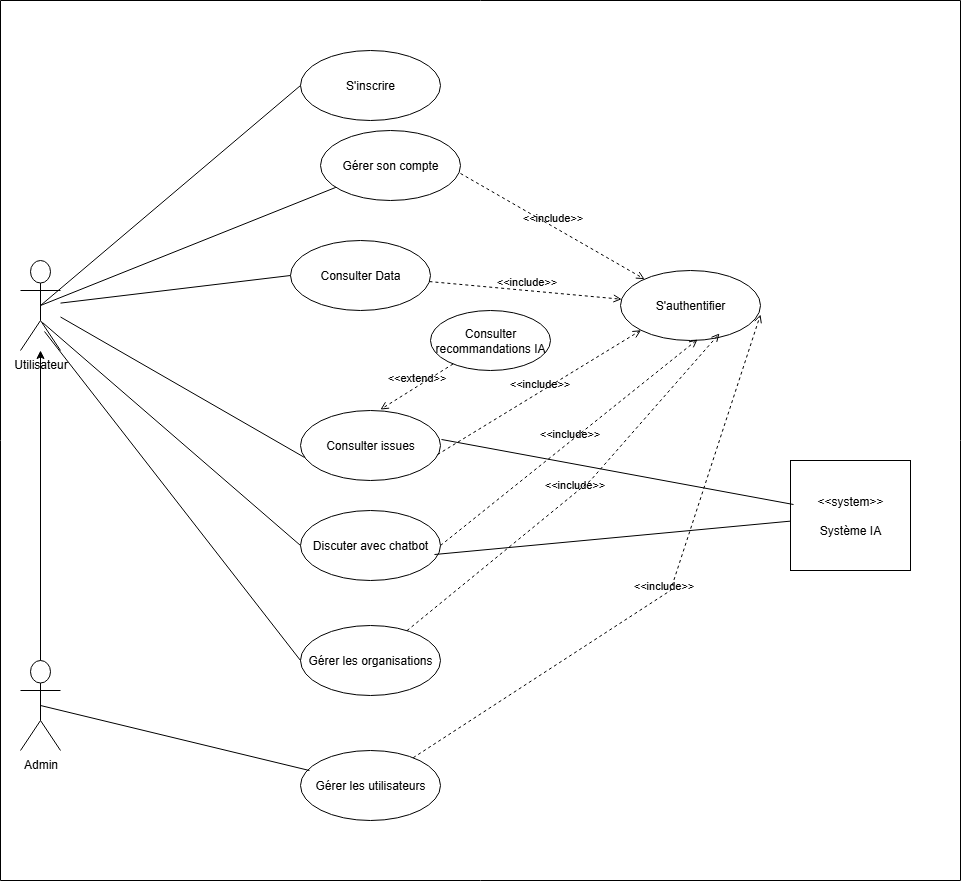
\includegraphics[width=1\linewidth]{img/useCaseGlobalFV.png}
    \caption{Diagramme de cas d’utilisation global}
    \label{fig:use-case}
\end{figure}

\section{Diagramme de classes global}
Le diagramme de classe permet de présenter les classes et les interfaces des systèmes, ainsi que les différentes relations qui les relient.

La figure 2.2  représente le diagramme de classes 
\begin{figure}[H]
    \centering
    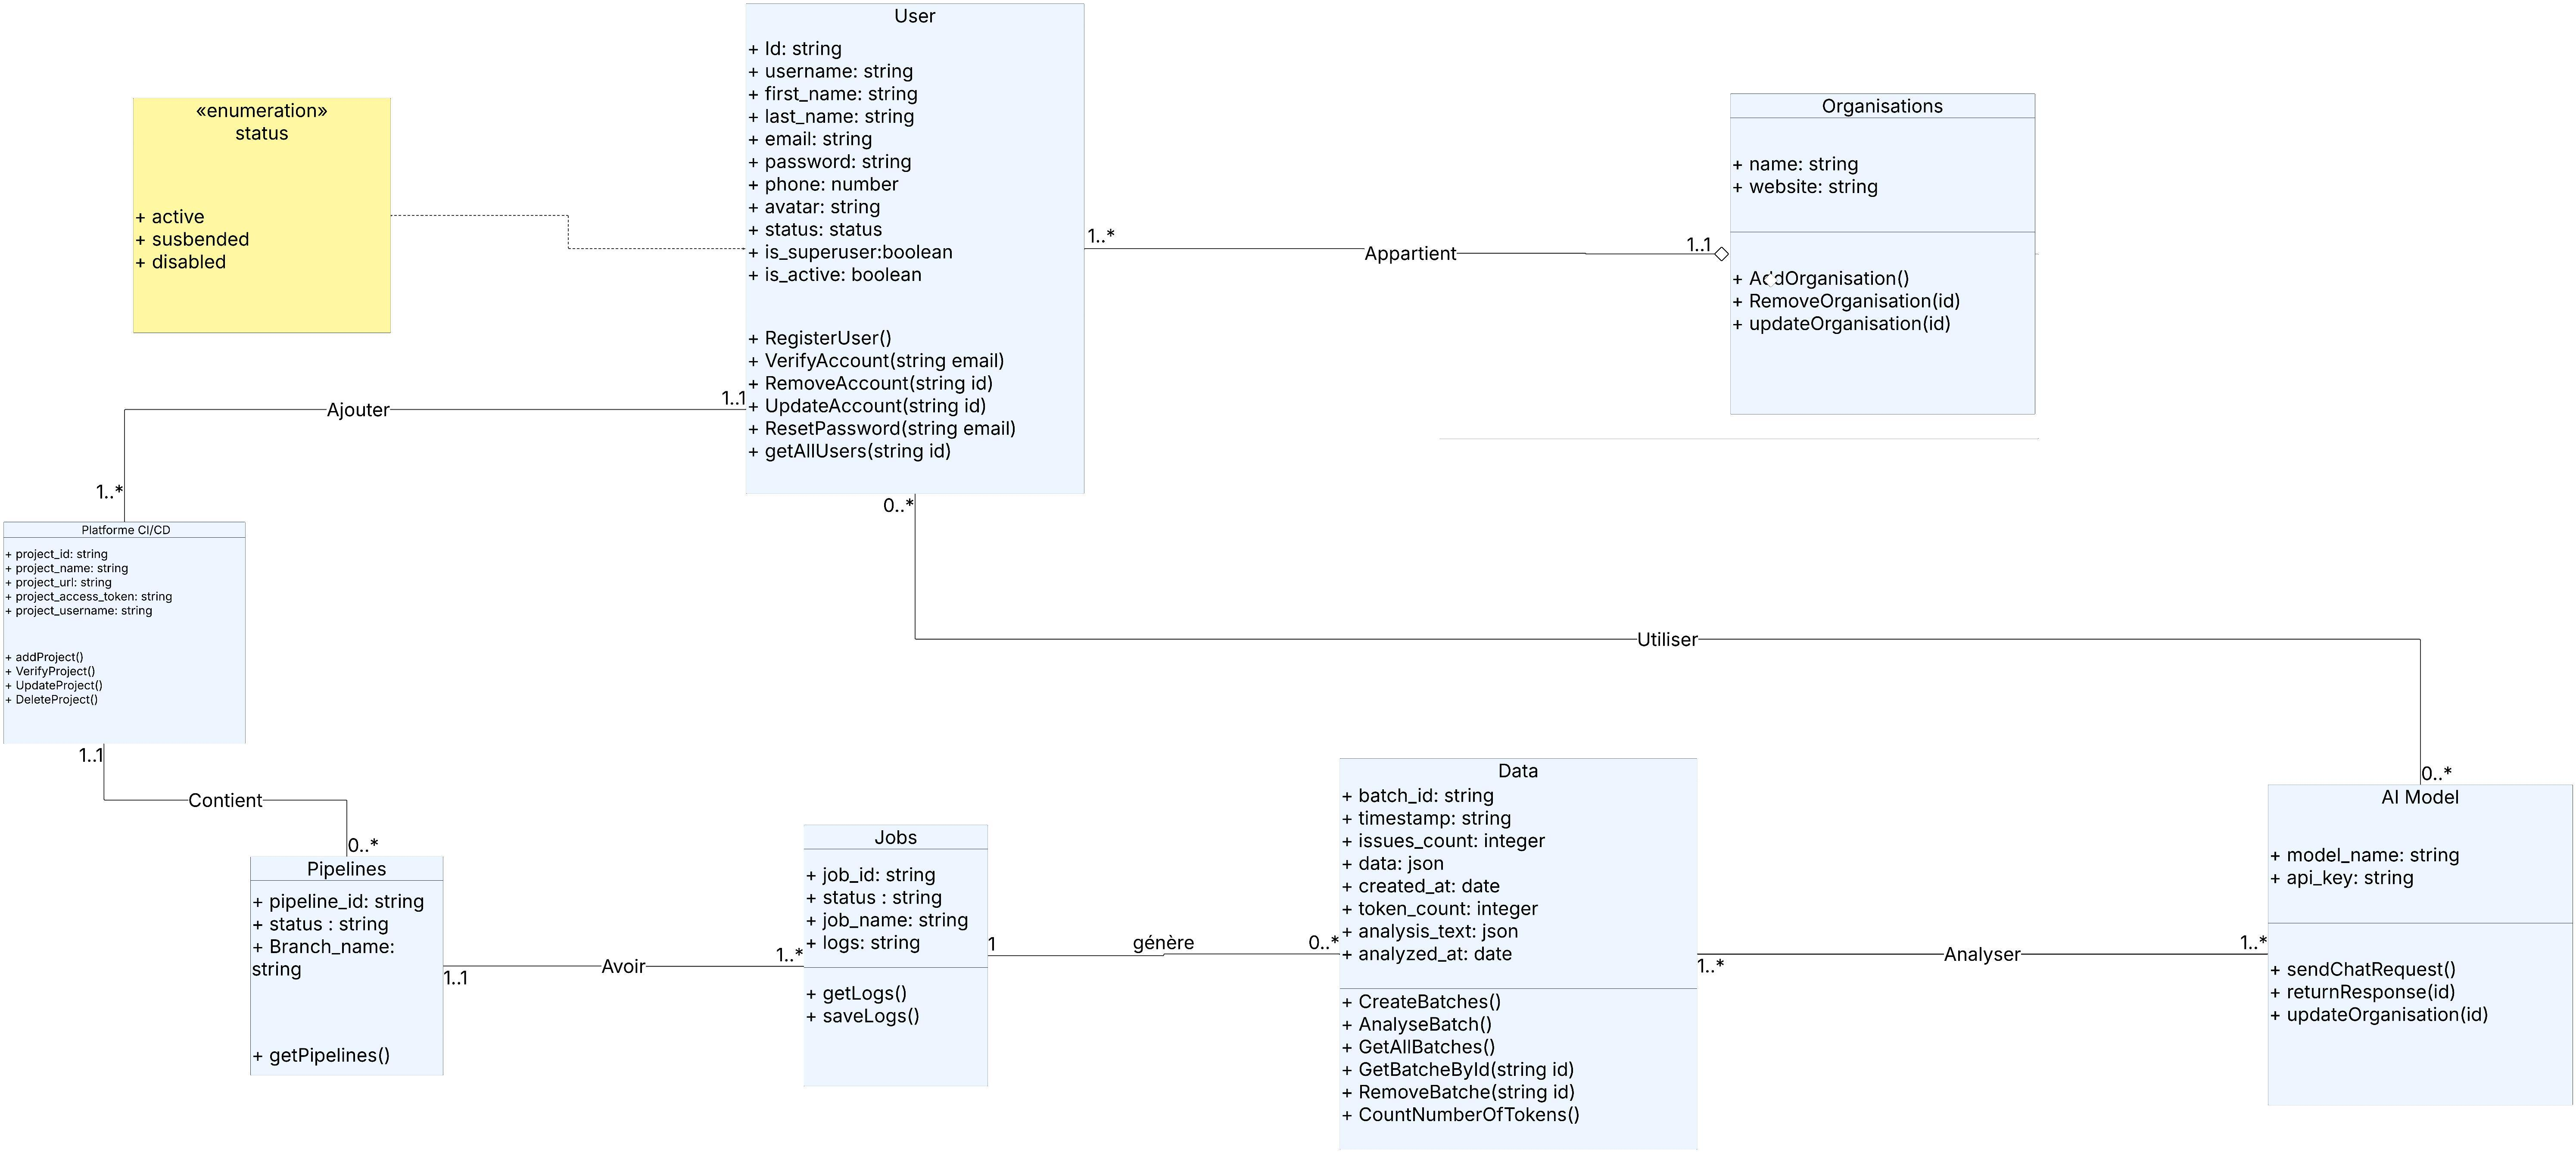
\includegraphics[width=1.2\linewidth]{img/Classes diagram global.jpeg}
    \caption{Diagramme de classes}
    \label{fig:use-case}
\end{figure}


\section{Pilotage du projet avec SCRUM}
\subsection{Identification de l’équipe SCRUM}

\begin{itemize}[label=\textbullet]
    \item \textbf{Product Owner :} Monsieur AYWANI Abdelmalek
    \item \textbf{Scrum Master :} Monsieur TELMOUDI Anes
    \item \textbf{Développeur  :} Ben Hassan Abdelkader 
    
\end{itemize}

\subsection{Backlog de Produit}
Le backlog est une liste priorisée des fonctionnalités à réaliser afin de répondre aux besoins des utilisateurs et aux objectifs du projet.
 
Pour estimer la complexité des éléments du backlog, nous avons adopté la méthode \textit{T-shirt sizing}, 
qui permet de classer les tâches selon leur niveau de difficulté ou d’effort attendu.  
Les valeurs utilisées sont :  

\begin{itemize}[label=\textbullet]
    \item \textbf{XS (Très simple)} : tâche rapide, faible effort.  
    \item \textbf{S (Simple)} : tâche de faible complexité, facilement réalisable.  
    \item \textbf{M (Moyenne)} : tâche nécessitant un effort modéré et une planification.  
    \item \textbf{L (Complexe)} : tâche assez lourde, impliquant plus de temps et de coordination.  
    \item \textbf{XL (Très complexe)} : tâche critique, à forte incertitude, demandant beaucoup de ressources.
\end{itemize}

{\scriptsize
\begin{longtable}{|
>{\centering\arraybackslash}m{0.7cm}|
>{\centering\arraybackslash}m{2.2cm}|
>{\centering\arraybackslash}m{1cm}|
m{5cm}|
>{\centering\arraybackslash}m{1cm}|
>{\centering\arraybackslash}m{1.3cm}|
>{\centering\arraybackslash}m{1.5cm}|}
\hline
\textbf{ID} & \textbf{Module} & \textbf{US ID} & \textbf{User Story} & \textbf{Prio.} & \textbf{Compl.} & \textbf{Nbr jours} \\
\hline
\endfirsthead

\hline
\textbf{ID} & \textbf{Module} & \textbf{US ID} & \textbf{User Story} & \textbf{Prio.} & \textbf{Complexité} & \textbf{Nombre jours} \\
\hline
\endhead

\multirow{7}{*}{1} & \multirow{7}{2.2cm}{Inscription \& Authentification} 
& 1.1 & En tant qu'admin, je veux créer un compte. & Élevée & M & 4 \\
\cline{3-7}
& & 1.2 & En tant qu'utilisateur, je veux créer un compte. & Moyenne & M & 3 \\
\cline{3-7}
& & 1.3 & En tant qu'admin, je veux m'authentifier pour accéder à mon espace. & Élevée & M & 5 \\
\cline{3-7}
& & 1.4 & En tant qu'utilisateur, je veux m'authentifier. & Moyenne & S & 3 \\
\cline{3-7}
& & 1.5 & En tant qu'utilisateur, je veux vérifier mon compte via email. & Moyenne & M & 3 \\
\cline{3-7}
& & 1.6 & En tant qu'utilisateur, je veux réinitialiser mon mot de passe. & Moyenne & M & 4 \\
\cline{3-7}
& & 1.7 & En tant qu'utilisateur, je veux recevoir un email de confirmation. & Moyenne & M & 3 \\
\hline

\multirow{3}{*}{2} & \multirow{3}{2.2cm}{Gestion des organisations} 
& 2.1 & En tant qu'admin, je veux consulter la liste des organisations. & Moyenne & M & 4 \\
\cline{3-7}
& & 2.2 & En tant qu'admin, je veux supprimer une organisation. & Moyenne & M & 3 \\
\cline{3-7}
& & 2.3 & En tant qu'admin, je veux modifier ou ajouter une organisation. & Moyenne & M & 4 \\
\hline

\multirow{2}{*}{3} & \multirow{2}{2.2cm}{Accès aux données} 
& 3.1 & En tant qu'utilisateur, je veux visualiser les logs et métriques en temps réel. & Élevée & XL & 20 \\
\cline{3-7}
& & 3.2 & En tant qu'utilisateur, je veux consulter la liste des batchs analysés. & Élevée & L & 10 \\
\hline

\multirow{3}{*}{4} & \multirow{3}{2.2cm}{Intégration du modèle IA} 
& 4.1 & En tant qu'utilisateur, je veux poser des questions sur un incident. & Élevée & M & 3 \\
\cline{3-7}
& & 4.2 & En tant qu'utilisateur, je veux discuter librement avec le chatbot. & Élevée & M & 3 \\
\cline{3-7}
& & 4.3 & En tant qu'utilisateur, je veux recevoir des recommandations. & Élevée & M & 3 \\
\hline

\multirow{2}{*}{5} & \multirow{2}{2.2cm}{Accès aux issues} 
& 5.1 & En tant qu'utilisateur, je veux consulter les anomalies détectées. & Élevée & M & 4 \\
\cline{3-7}
& & 5.2 & En tant qu'utilisateur, je veux voir les recommandations de l'IA. & Élevée & M & 4 \\
\hline

\multirow{2}{*}{6} & \multirow{2}{2.2cm}{Intégration des projets} 
& 6.1 & En tant qu'utilisateur, je veux ajouter des projets depuis GitLab. & Élevée & L & 5 \\
\cline{3-7}
& & 6.2 & En tant qu'utilisateur, je veux consulter les logs des pipelines CI/CD. & Élevée & XL & 10 \\
\hline

\multirow{4}{*}{7} & \multirow{4}{2.2cm}{Gestion des utilisateurs} 
& 7.1 & En tant qu’administrateur, je veux attribuer ou modifier les rôles des utilisateurs . & Élevée & M & 3 \\
\cline{3-7}
& & 7.2 & En tant qu’administrateur, je veux gérer les états des utilisateurs (actif, inactif, suspendu) pour contrôler l’accès au système. & Faible & L & 4 \\
\cline{3-7}
& & 7.3 & En tant qu’administrateur, je veux modifier les informations des utilisateurs. & Faible & M & 2 \\
\cline{3-7}
& & 7.4 & En tant qu’administrateur, je veux supprimer des utilisateurs. & Élevée & M & 2 \\
\hline

\captionsetup{justification=centering}
\caption{Backlog produit}
\label{tab:backlog}
\end{longtable}
}

Le tableau 2.2 représente le Backlog de produit.

\subsection{Répartition des Sprints en release}
L’adoption de la méthode Scrum implique de diviser le projet en sprints. Une release correspond à la livraison d’une version aboutie du produit. Elle désigne la période allant du lancement des travaux jusqu’à la mise à disposition du livrable, comprenant une succession de sprints. Dans notre cas, nous avons structuré notre projet en quatre releases.

Le tableau 2.3 montre comment les sprints sont répartis et combien de jours sont estimés pour chaque sprint.
\begin{table}[H]
\centering
\renewcommand{\arraystretch}{1.4}
\begin{tabular}{|
>{\centering\arraybackslash}m{3cm}|
>{\centering\arraybackslash}m{3cm}|
m{7cm}|
>{\centering\arraybackslash}m{3cm}|}
\hline
\textbf{Releases} & \textbf{Sprints} & \textbf{Fonctionnalités du Sprint} & \textbf{Estimation en nombre de jours} \\
\hline

\multirow{2}{*}{Release 1} 
& Sprint 1 
& - Module d’authentification \newline - Gestion du profil \newline - Gestion des organisations \newline - Réinitialisation du mot de passe \newline - Vérification du compte 
& 20 jours \\
\cline{2-4}

& Sprint 2 
& - Création des batches \newline - Gestion des logs \newline - Gestion des métriques 
& 30 jours \\
\hline

\multirow{2}{*}{Release 2}
& Sprint 3 
& - Intégration du modèle IA
& 20 jours \\
\cline{2-4}

& Sprint 4
& - Analyse des logs et des métriques 
& 30 jours \\
\hline


\multirow{2}{*}{Release 3}
& Sprint 5
& - Gestion des projets 
& 25 jours \\
\cline{2-4}

& Sprint 6 
& - Gestion des utilisateurs 
& 15 jours \\
\hline

\end{tabular}
\captionsetup{justification=centering}
\caption{Plan des Releases et Sprints avec estimations en jours}
\label{tab:releases-sprints}
\end{table}



\section{Architecture de l’application}

\subsection{Architecture logique}
Notre projet est basé sur l'architecture MVC (Modèle–Vue–Contrôleur), qui vise à séparer clairement trois aspects fondamentaux d’une application : les données (modèle), l’interface utilisateur (vue) et la logique de traitement (contrôleur).

Cette architecture s’organise autour de trois couches distinctes :
\begin{itemize} [label=\textbullet]
  
\item \textbf {Modèle :} Il représente la structure des données de l’application, assure la gestion des interactions avec la base de données et le traitement des informations.

\item \textbf  {Vue :} Elle correspond à l’interface utilisateur. Son rôle se limite à l’affichage des données transmises par le modèle, sans y appliquer de traitement.

\item \textbf  {Contrôleur :} Il fait le lien entre le modèle et la vue. Il interprète les requêtes de l’utilisateur, sélectionne la vue adéquate à afficher, et coordonne la synchronisation entre les données et l’affichage.
\end{itemize}

\begin{figure}[H]
    \centering
    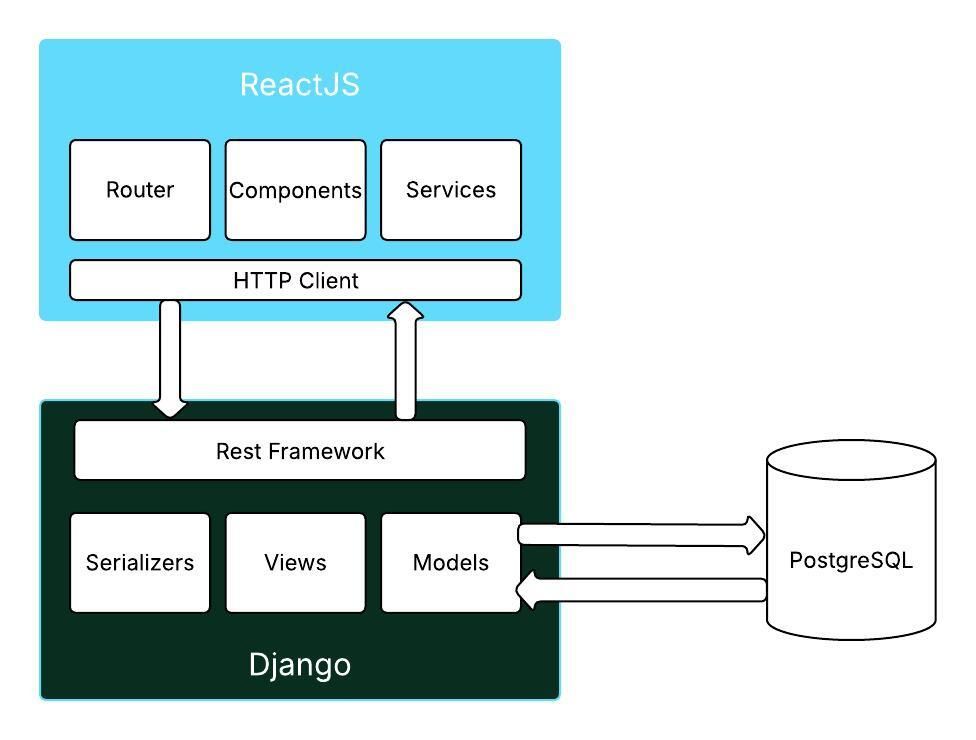
\includegraphics[width=0.85\linewidth]{img/archilogique.jpeg}
    \caption{Architecture logique}
    \label{fig:use-case}
\end{figure}



\subsection{Architecture physique}
L’architecture adoptée pour notre application est celle en N-tier illustrée par la figure 2.3
(client, serveur web, serveur applicatif, serveurs de bases de données). 
Cette approche permet
de diviser l’application en plusieurs niveaux de services distincts, conformément aux principes
suivants :

\begin{itemize}
 
\item  \textbf{Le Client : } C’est la couche où l’utilisateur interagit directement avec l’application via un navigateur
web. La couche cliente consomme les interfaces offertes par le serveur React Js pour présenter les
données et permettre les interactions avec l’utilisateur.

\item  \textbf {Le serveur Web : } Cette couche sert d’intermédiaire entre le client et l’application. Elle reçoit les
requêtes des clients, les transmet aux serveurs d’application appropriés, et renvoie les réponses aux
clients.

\item  \textbf {Le serveur applicatif :} Cette couche correspond au serveur back-end, développé en Django (REST
API). Elle reçoit les requêtes envoyées par le client (React Js), traite les logiques métier, effectue
les analyses et communique avec les serveurs de bases de données. C’est aussi ici que les services
d’analyse IA sont intégrés.

\item  \textbf {Les serveurs de bases de données :} Cette couche est responsable de la gestion des données. Elle
stocke les données de l’application de manière structurée et permet leur accès et leur manipulation.

\begin{itemize} [label=\textbullet]
    \item  \textbf{PostgreSQL :} Utilisé pour gérer les données internes de l’application telles que les utilisateurs, les projet ci/cd, les batches et les session des chat avec l'IA.
 \item  \textbf {TimescaleDB :} utilisé pour stocker les métriques du cpu , mémoire du serveur cloud.
 \item  \textbf {Elasticsearch :} Indexation et recherche des logs.
\end{itemize}
\end{itemize}

\begin{figure}[H]
    \centering
    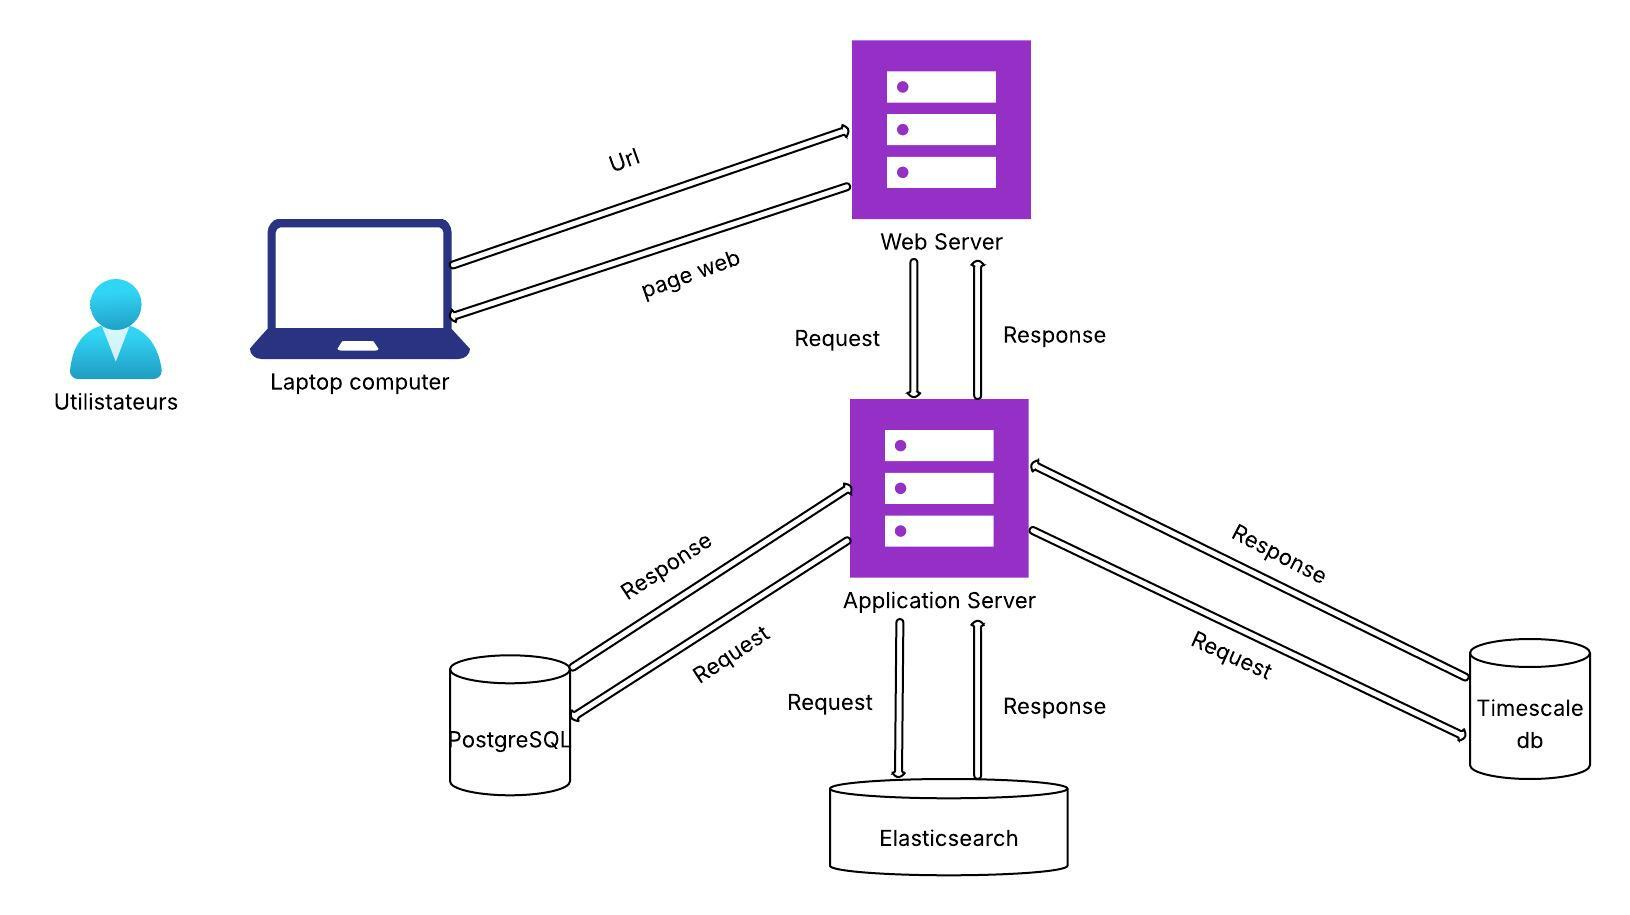
\includegraphics[width=0.85\linewidth]{img/architecture physique.jpeg}
    \caption{Architecture physique}
    \label{fig:use-case}
\end{figure}

\section{Environnement de travail}

\subsection{Environnement matériel}
Pendant ce stage, nous avons utilisé un ordinateur portable pour développer notre application, dont les caractéristiques seront exposées dans ce tableau : 

\begin{table}[H]
\centering
\begin{tabular}{|l|l|}
\hline
\textbf{Caractéristique}        & \textbf{Détail}                         \\ \hline
Processeur                      & AMD Ryzen 5 5500U 2.10 GHZ                    \\ \hline
Mémoire RAM                    & 20 Go DDR4                  \\ \hline
Stockage                        & SSD de 512 Go                           \\ \hline

Système d’exploitation          & Windows 11 Pro                         \\ \hline
\end{tabular}
\captionsetup{justification=centering}
\caption{Caractéristiques du poste de travail utilisé}
\label{tab:environnement matériel}
\end{table}


\subsection{Environnement logiciel}
Pour atteindre les objectifs de notre projet, nous avons utilisé les outils suivants :

\begin{itemize}[label=\textbullet]
\item \textbf{Visual Studio Code :} est un éditeur de code source gratuit et open source développé par Microsoft. Il est largement utilisé par les développeurs pour écrire, modifier et gérer du code dans différents langages de programmation.

\begin{figure}[H]
    \centering
    
\includegraphics[width=0.25\linewidth]{img/vscode.png}
    \caption{Logo Vs Code}
    \label{fig:enter-label}
\end{figure}

\item \textbf{Python:} Python est un langage de programmation interprété, haut niveau et généraliste, réputé pour sa simplicité, sa lisibilité et sa facilité d’apprentissage. Il supporte plusieurs paradigmes de programmation, notamment la programmation impérative, orientée objet et fonctionnelle.

\begin{figure}[H]
    \centering
    
\includegraphics[width=0.25\linewidth]{img/python.jpeg}
    \caption{Logo Python}
    \label{fig:enter-label}
\end{figure}


\item \textbf{Django :} est un framework web open source écrit en Python. Il facilite et accélère le développement d’applications web en fournissant une structure prête à l’emploi qui suit le principe "batteries included" (tout est inclus).

\begin{figure}[H]
    \centering
    
\includegraphics[width=0.25\linewidth]{img/django.png}
    \caption{Logo Django}
    \label{fig:enter-label}
\end{figure}

\item \textbf{ReactJs :} est une bibliothèque JavaScript développée par Facebook pour construire des interfaces utilisateur interactives, surtout des applications web à page unique (SPA). Elle repose sur un concept de composants réutilisables et un DOM virtuel pour optimiser les mises à jour de l’affichage.

\begin{figure}[H]
    \centering
    
\includegraphics[width=0.25\linewidth]{img/reactjs.png}
    \caption{Logo ReactJs}
    \label{fig:enter-label}
\end{figure}

\item \textbf{Docker :} est une plateforme qui permet de créer, déployer et exécuter des applications dans des conteneurs légers et portables. Ces conteneurs emballent une application avec toutes ses dépendances pour garantir qu’elle fonctionne de la même façon partout, que ce soit sur un poste de travail, un serveur ou dans le cloud..

\begin{figure}[H]
    \centering
    
\includegraphics[width=0.25\linewidth]{img/docker.png}
    \caption{Logo Docker}
    \label{fig:enter-label}
\end{figure}

\item \textbf{Fluentd :} st un outil open source de collecte, transformation et routage des logs et des données de streaming. Il agit comme un collecteur unifié pour centraliser les logs provenant de différentes sources et les envoyer vers des destinations variées (bases de données, moteurs de recherche, systèmes de stockage…).

\begin{figure}[H]
    \centering
    
\includegraphics[width=0.25\linewidth]{img/fluentd.png}
    \caption{Logo Fluentd}
    \label{fig:enter-label}
\end{figure}

\item \textbf{Elasticsearch :} est un moteur de recherche et d’analyse distribué basé sur Lucene. Il permet de stocker, rechercher et analyser de grandes quantités de données rapidement, souvent utilisé pour des applications de recherche textuelle, d’analyse de logs et de données en temps réel.

\begin{figure}[H]
    \centering
    
\includegraphics[width=0.25\linewidth]{img/elastic.png}
    \caption{Logo Elasticsearch}
    \label{fig:enter-label}
\end{figure}


\item \textbf{PostgreSQL :}est un système de gestion de base de données relationnelle (SGBDR) open source, robuste et puissant. Il supporte les transactions complexes, l’intégrité référentielle, et propose des fonctionnalités avancées comme les types de données personnalisés, les vues, les déclencheurs, et plus.

\begin{figure}[H]
    \centering
    
\includegraphics[width=0.25\linewidth]{img/PostgreSQL.png}
    \caption{Logo PostgreSQL}
    \label{fig:enter-label}
\end{figure}

\item \textbf{TimescaleDB :} est une extension de PostgreSQL optimisée pour le stockage et l’analyse des données temporelles (time-series data). Elle facilite la gestion efficace de grandes quantités de données horodatées, souvent utilisées dans les domaines de l’IoT, la finance, la surveillance et la télémétrie.

\begin{figure}[H]
    \centering
    
\includegraphics[width=0.25\linewidth]{img/timescale.png}
    \caption{Logo TimescaleDB}
    \label{fig:enter-label}
\end{figure}

\item \textbf{Jira :} est un système de suivi des bugs, de gestion des incidents et de gestion de projets développé par Atlassian et publié pour la première fois en 2002. Il propose des solutions à la fois à destination des développeurs et des intervenants non développeurs.

\begin{figure}[H]
    \centering
    
\includegraphics[width=0.25\linewidth]{img/jira.jpg}
    \caption{Logo Jira}
    \label{fig:enter-label}
\end{figure}

\end{itemize}

\section{Conclusion}
Dans ce chapitre, nous avons présenté une analyse approfondie du système, ses acteurs, ses besoins fonctionnels et non fonctionnels, les cas d'utilisation ainsi que la méthode de pilotage Scrum adoptée. Cette phase est primordiale pour assurer une conception et un développement structurés et efficaces de l’application.
